\documentclass[a0paper,portrait,fleqn,leqno]{tikzposter}
% Ein Blatt in DIN A0 ist 841 mm breit und 1189 mm lang
\title{Wegfindung im Labyrinth}
\institute{Universit\"{a}t Heidelberg}
\author{Florian Nowak \& Yichuan Shen}
%\author{%
%  Florian Nowak\footnote{Florian Nowak: B.\,Sc. Mathematik, 7. Fachsemester}\; \& Yichuan Shen\footnote{Yichuan Shen: M.\,Sc. Mathematik, 1. Fachsemester}\\
%  Betreuer: Gero Plettenberg, Thomas Kloepfer
%  }
\date{Wintersemester 2014/15}

% Für die Bestimmungen aus dem Leitfaden siehe Dokumentende

\settitle{%
  \vspace*{2cm}
  \color{titlefgcolor}%
  \begin{minipage}[t]{.48\textwidth}
  \begin{flushright}
  {\bfseries\Huge\sc\@title}\hspace*{2cm}\par%
  \vspace*{1cm}%
  {\huge\@author\hspace*{2cm}}\par%
  \vspace*{1cm}
  {\LARGE\@institute\hspace*{2cm}}\par%
  \vspace*{.5cm}
  \raisebox{-4mm}{{\Large\@date\hspace*{2cm}}}\par%
  \end{flushright}
  \end{minipage}%
  \begin{minipage}{.48\textwidth}
  \begin{flushleft}
  \hspace*{2cm}\@titlegraphic
  \end{flushleft}
  \end{minipage}
  }

\tikzposterlatexaffectionproofoff
  
%\settitle{ \centering \vbox{
%\@titlegraphic \\[\TP@titlegraphictotitledistance] \centering
%\color{titlefgcolor} {\bfseries \Huge \sc \@title \par}
%\vspace*{1em}
%{\huge \@author \par} \vspace*{1em} {\LARGE \@institute}
%}}
  
\colorlet{Gray}{black!40}
\colorlet{lightGray}{black!25}
\colorlet{Lime}{lime!50!black!70}
\colorlet{lightLime}{lime!50!black!30}
%\colorlet{Blue}{blue!50!black!70}
\definecolor{Blue}{HTML}{304664}

\definecolorstyle{mystyle}{%
  \definecolor{colorOne}{named}{lightGray}
  \definecolor{colorTwo}{named}{Blue}
  }{%
  % Background Colors
  \colorlet{backgroundcolor}{white}
  \colorlet{framecolor}{colorOne}
  % Title Colors
  \colorlet{titlefgcolor}{black}
  \colorlet{titlebgcolor}{white}
  % Block Colors
  \colorlet{blocktitlebgcolor}{colorTwo}
  \colorlet{blocktitlefgcolor}{white}
  \colorlet{blockbodybgcolor}{white}
  \colorlet{blockbodyfgcolor}{black}
  }
\definelayouttheme{mytheme}{%
  \usecolorstyle{mystyle}
  \usebackgroundstyle{Default} 
  % Predefined Styles: Default, Rays, VerticalGradation, 
  % BottomVerticalGradation, Empty
  \usetitlestyle{Filled} 
  % Default, Basic, Envelope, Wave, VerticalShading, Filled, Empty
  \useblockstyle{Basic}
  % Default, Basic, Minimal, Envelope, Corner, Slide, TornOut
  \useinnerblockstyle{Default} 
  % Default, Table
  \usenotestyle{Sticky} 
  % Default, Corner, VerticalShading, Sticky
  }

\titlegraphic{%
  \includegraphics[width=19cm]{orb}
  % Die Breite des Logos beträgt a + c + c + a = 140,2 mm + 10 mm + 10 mm + 140,2 mm = 300,4 mm für Anwendungen in DIN A0 (siehe Gestaltungshandbuch, Seite 11). Der Abstand des Logos zum oberen sowie zum rechten Rand des Posters beträgt c + d = 10 mm + 20 mm = 30 mm.
  }
\usetheme{mytheme}

\usepackage[ngerman]{babel}
\usepackage{graphicx}
\usepackage[colorlinks=true,urlcolor=cyan,hidelinks]{hyperref}
\usepackage[utf8]{inputenc}
\usepackage[default]{sourcesanspro}
\usepackage{amssymb}

%\usepackage{minted}
%  \usemintedstyle{monokai}
\usepackage{blindtext}


\begin{document}
\maketitle


\begin{columns}
  \column{.5}
  \block[roundedcorners=0,linewidth=2pt]{Aufgabenstellung}{%
  \begin{tikzfigure}%[Roboter mit aufliegendem Labyrinth]
  	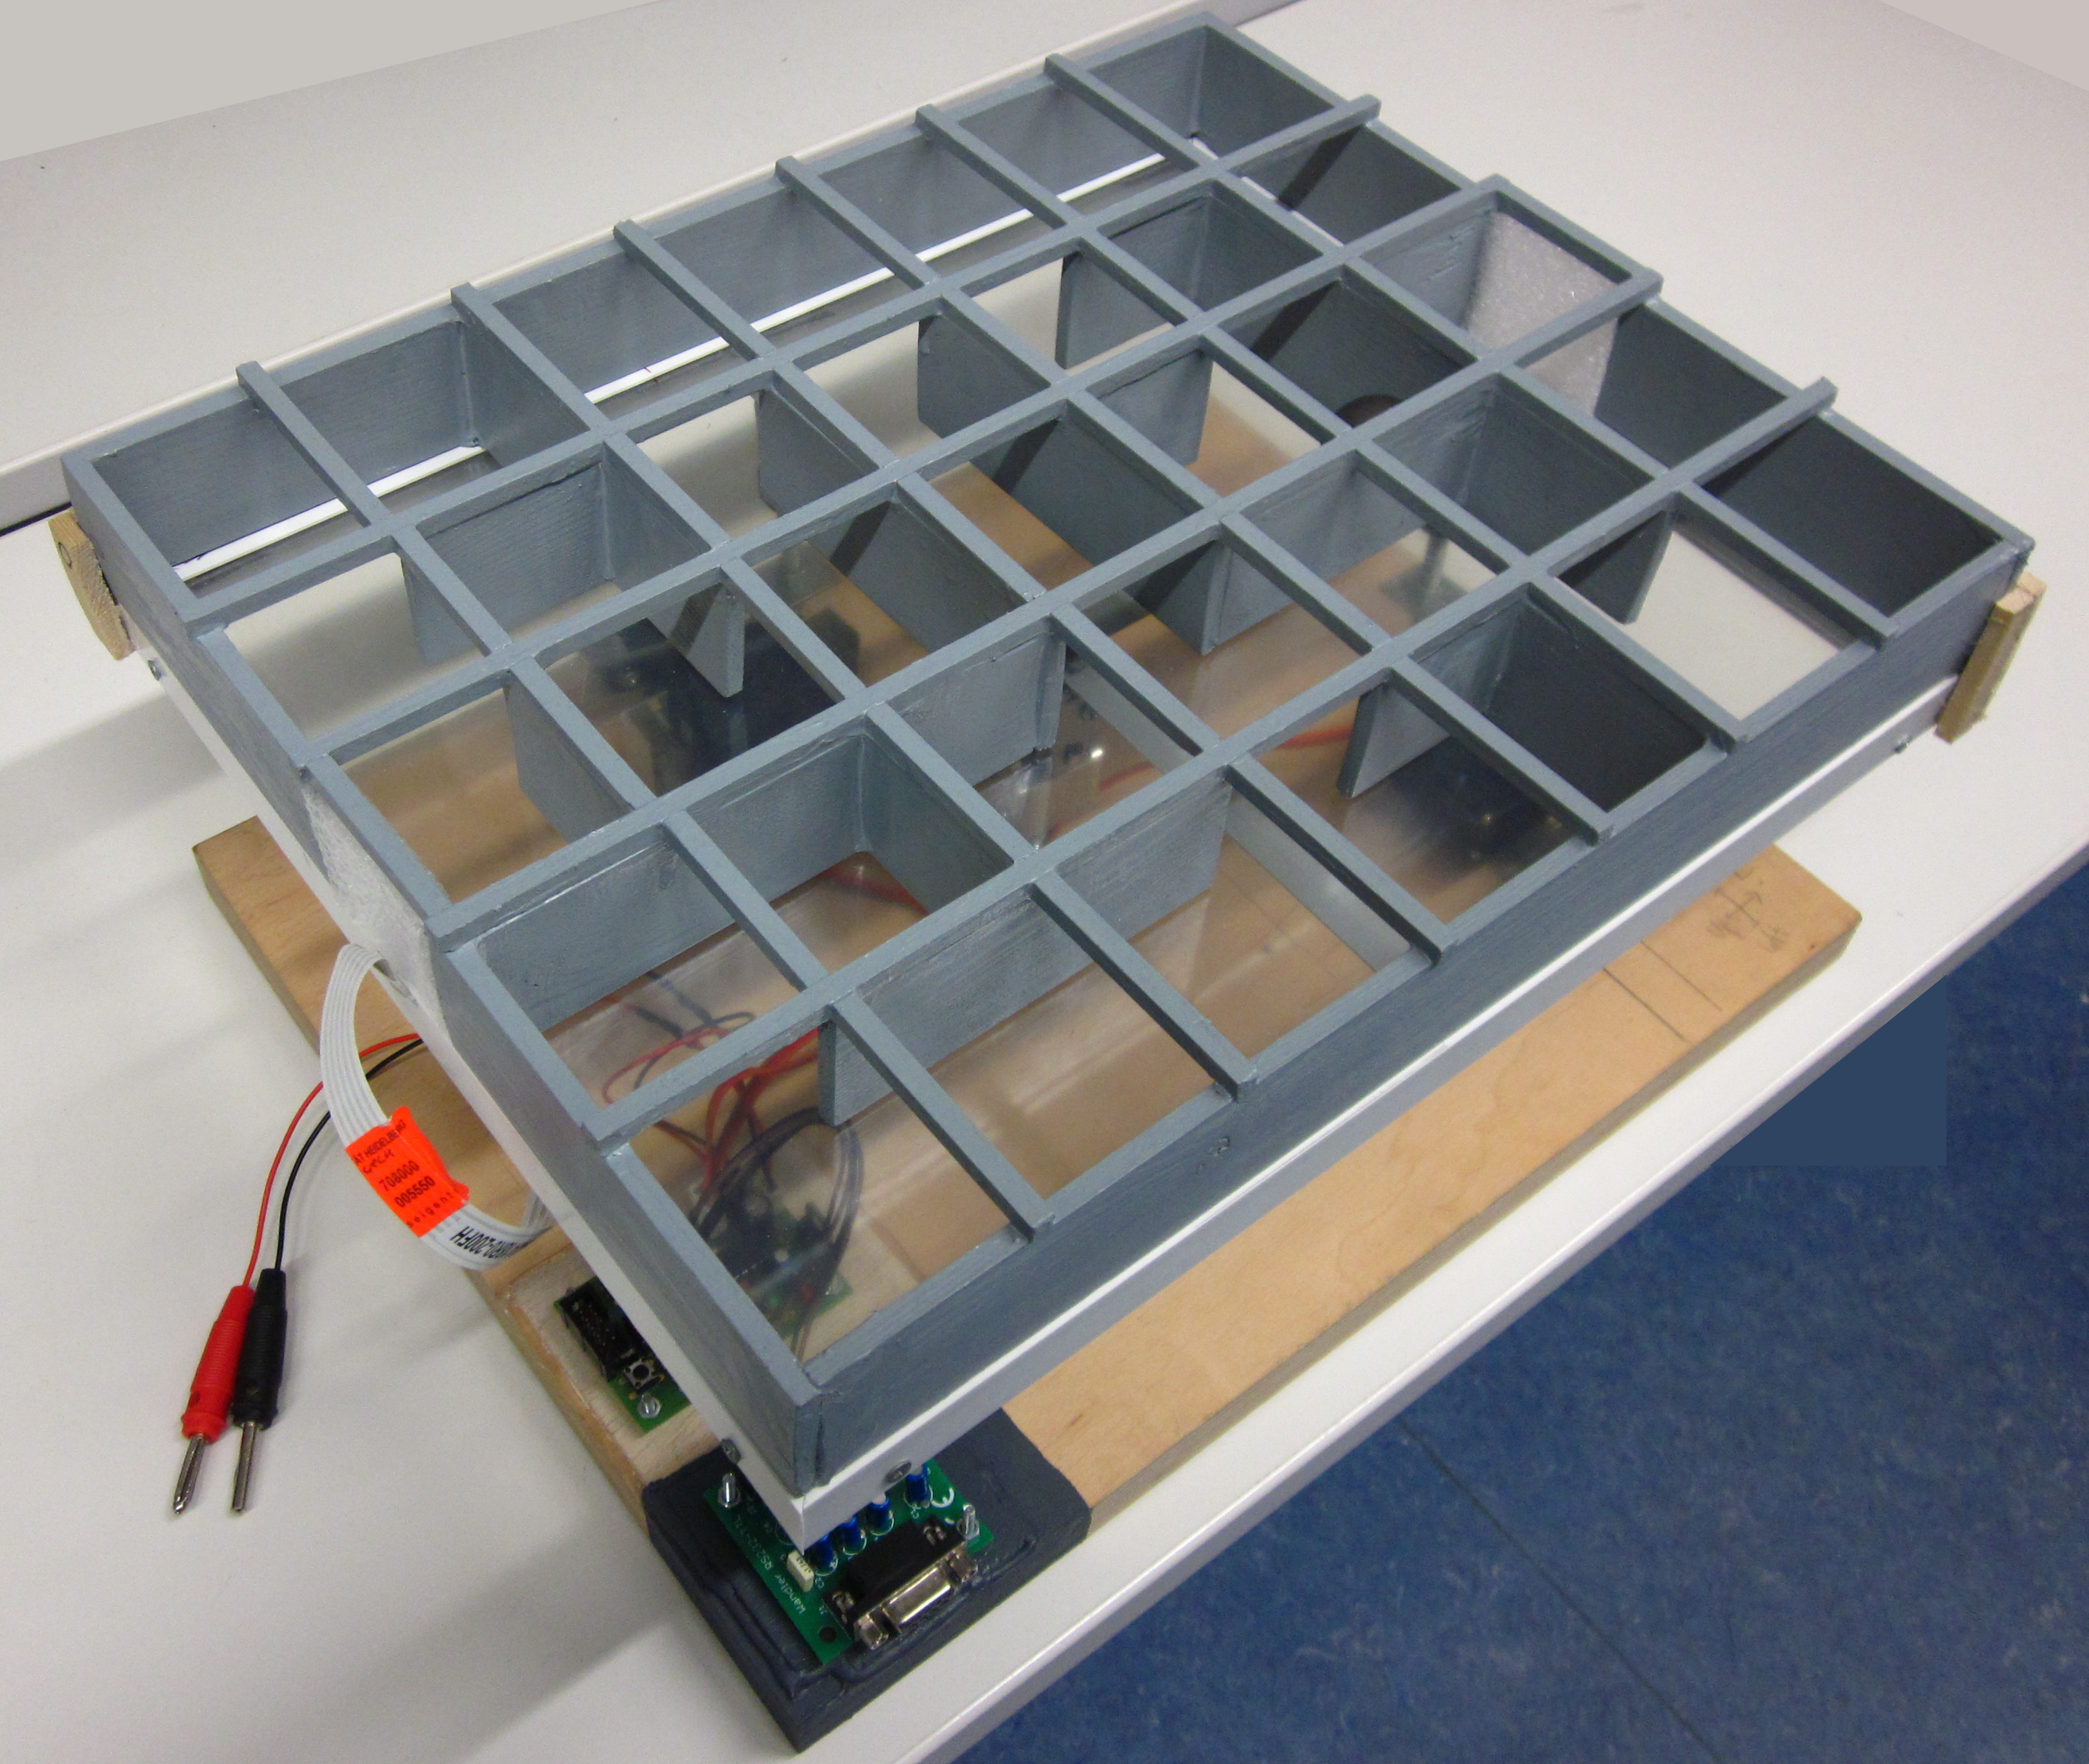
\includegraphics[width=38cm]{roboter_badly-photoshoped}
  \end{tikzfigure}
  \vspace{1em}
  Ein bereits vorhandener Roboter mit neigbarem Touchscreen soll etwas Neues lernen: 
  
  \smallskip\noindent
  Er soll ein beliebiges auf dem Rahmen seines Touchscreens aufliegendes Labyrinth (vorgegebener Rastergröße) mithilfe einer Metallkugel einlesen können. Der Roboter kann eine solche Kugel bereits auf eine ihm vorgegebene Richtung durch Kippen rollen lassen und dort ausbalancieren, so dass die Kugel stillsteht. Das Roboter soll zudem ein zuvor eingelesenes Labyrinth mit der Kugel auf optimalem Weg lösen können.
  
  \bigskip\noindent
  \textbf{Vereinfachungen:}  
  \begin{itemize}
  \item[\raisebox{.35ex}{\tiny$\blacksquare$}] Das Labyrinth soll rechteckig und \emph{gleichmäßig} sein.
  \item[\raisebox{.35ex}{\tiny$\blacksquare$}] Die Maße des Labyrinths werden als bekannt vorausgesetzt.
  \end{itemize}
  }
  \block[roundedcorners=0,linewidth=2pt]{Ergebnis}{%
  Obwohl der Roboter für die Wanderkennung jedes Feld des Labyrinths ansteuern muss, braucht die Erkennung des gesamten Testlabyrinths (35 Felder) dank diverser Optimierungen lediglich etwas mehr als 10 Minuten. Zudem kann man das erkannte Labyrinth in einer Datei speichern und es zu einem späteren Zeitpunkt lösen lassen.
  }
  {\colorlet{framecolor}{white}
  \block{}{%
  \includegraphics[width=38cm]{mcu-kabel_2}
  }}
%  \block[roundedcorners=0,linewidth=2pt]{Sonstiges}{%
%  \textbf{GitHub Projektseite:}\hspace{1em}\url{github.com/flo7210/WegfLaby_AP} 
%  }
  \column{.5}
  \block[roundedcorners=0,linewidth=2pt]{Labyrintherkennung}{%
  Beim Erkennen des Labyrinths besteht die Herausforderung im Wesentlichen aus der \emph{(lokalen) Wanderkennung}: Für ein Feld soll überprüft werden, ob die benachbarten Felder mit der Kugel erreichbar sind. Die Labyrintherkennung ist schließlich eine Iteration über die Wanderkennung bei jedem Feld.

\smallskip\noindent
Das Lösen des Labyrinths ist anschließend lediglich eine Breitensuche.
  }
  \block[roundedcorners=0,linewidth=2pt]{Wanderkennung}{%
  Das folgende Flowchart stellt die Wanderkennung für ein bestimmtes Feld \texttt{anchor} im Labyrinth dar. Dabei enthält \texttt{neighbors{\textunderscore}stack} alle benachbarten Felder von \texttt{anchor}, deren lokale Wanderkennung noch aussteht.
  \vspace{1em}
  \begin{tikzfigure}
  	\includegraphics[width=38cm]{flowchart_cutout}
  \end{tikzfigure}
  }
  \block[roundedcorners=0,linewidth=2pt]{Festhalten des Fortschritts}{%
  Der Roboter fängt mit der Labyrintherkennung bei einem beliebigen Feld an. Nach der Wanderkennung beim Anfangsfeld erhalten wir dessen erreichbare benachbarten Felder und speichern davon diejenigen Felder in einem globalen Stack, deren Wanderkennung noch aussteht. Es wird ein Feld aus dem Stack gewählt und entfernt. Nun wird die Kugel zum gewählten Feld geschickt und die ganze Prozedur solange wiederholt bis der Stack leer ist.
  }
  \block[roundedcorners=0,linewidth=2pt]{Optimierung}{%
  \begin{itemize}
  \item[\raisebox{.35ex}{\tiny$\blacksquare$}] Die Wanderkennung bei einem Punkt lässt die Kugel auf dem letzten überprüften Feld, falls dieses erreichbar war. Somit spart man sich ein unnötiges Zurückgehen zum Anker.
  \item[\raisebox{.35ex}{\tiny$\blacksquare$}] Falls die Kugel am Ende der Wanderkennung auf einem Nachbarfeld gelassen wurde, wird dieser bei der Wahl aus dem Stack bevorzugt.
  \end{itemize}
  }
  {\colorlet{framecolor}{white}
  \block{}{\vspace{3.855cm}}
  }
  \block[roundedcorners=0,linewidth=2pt]{Beteiligte}{%
  %\textbf{Studierende}\\
  \makebox[0pt][l]{\textbf{Florian Nowak:}}\hphantom{Gero Plettenberg}\hspace{1em}B.\,Sc. Mathematik, 7. Fachsemester\\
  \makebox[0pt][l]{\textbf{Yichuan Shen:}}\hphantom{Gero Plettenberg}\hspace{1em}M.\,Sc. Mathematik, 1. Fachsemester
  
  \medskip\noindent
  Gero Plettenberg\hspace{1em}\textit{(Betreuer)}\\
  \makebox[0pt][l]{Thomas Kloepfer}\hphantom{Gero Plettenberg}\hspace{1em}\textit{(Supervisor)} 
  
  \bigskip\noindent
  \textbf{GitHub Projektseite:}\hspace{1em}\url{github.com/flo7210/WegfLaby_AP}
  }
\end{columns}

\end{document}

% Auszug aus dem Leitfaden (Abschnitt 7.2):
%
% Das Poster dient dazu, das Ergebnis des Projektes auf eine prägnante und ansprechende Weise darzustellen. Im Gegensatz zur Webpage liegt der Fokus beim Poster auf dem Ergebnis des Praktikums und nicht auf dem Praktikumsverlauf. Das Layout des Posters soll gut strukturiert und optisch ansprechend sein. Zwischen Grafiken und Text soll ein Gleichgewicht herrschen und es soll sichergestellt sein, dass der Betrachter Grafiken dem zugehörigen Text zuordnen kann.
%
% Das Poster beinhaltet folgende Punkte:
% • Titel des Projektes
% • Bearbeitungszeitraum (das jeweilige Semester, in dem das Praktikum absolviert wurde)
% • Name und Studienfächer der Studierenden
% • Betreuer und Supervisor
% • Aufgabenstellung des Projektes
% • Ergebnis
% • Bilder des Roboters, Visualisierung o. Ä.
%
% Das Poster ist in DinA0- oder DinA4- Format als PDF dem jeweiligen Betreuer zu schicken. Auf ausreichende Auflösung der Fotos ist zu achten, außerdem sollten Texte und Graphiken im Vektorformat vorliegen. Die Hintergrundfarbe des Posters ist weiß.